\documentclass[a4paper,landscape,10pt]{article}
\usepackage[
  left=1.2cm,
  right=1.2cm,
  top=2.2cm,
  bottom=1.5cm,
  headheight=16pt,
  headsep=12pt
]{geometry}
\usepackage{longtable}
\usepackage{array}
\usepackage{xcolor}
\usepackage{helvet}
\usepackage{colortbl}
\usepackage{fancyhdr}
\usepackage[hidelinks]{hyperref}
\usepackage{graphicx}

\renewcommand{\familydefault}{\sfdefault}
\pagestyle{fancy}
\fancyhf{}
\rhead{\footnotesize \textbf{GEMASTIK XIX 2026} -- Divisi Pengembangan Perangkat Lunak -- Tim Three Achilles (TRPL SV UGM)}
\lhead{\footnotesize \textbf{Storyboard Video Karya Akhir 100\% (Opsi Referensi Baru)}: Verifin}
\rfoot{\footnotesize Halaman \thepage}

\setlength{\parindent}{0pt}
\renewcommand{\arraystretch}{1.25}
\setlength{\tabcolsep}{3.5pt}

% Custom column types with clean wrapping
\newcolumntype{C}[1]{>{\centering\arraybackslash}p{#1}}
\newcolumntype{L}[1]{>{\raggedright\arraybackslash}p{#1}}

\begin{document}

% Metadata Header
\noindent
\begin{minipage}[t]{0.68\textwidth}
{\large \textbf{GEMASTIK XIX 2026 -- Divisi Pengembangan Perangkat Lunak}} \\[0.15cm]
\small
\begin{tabular}{@{}lp{14.2cm}@{}}
\textbf{Pemeran (5)} & : 1. Rama (Alumni Muda), 2. Dr.Eng. Ir. Ganjar Alfian, S.T., M.Eng. (Dosen), 3. Matthew, 4. Hafidz, 5. Akmal (Three Achilles) \\
\textbf{Lokasi} & : \textbf{100\% Lingkungan Kampus} (Student Lounge, Selasar TILC, Ruang Dosen, \& Lab RPL TILC UGM) \\
\textbf{Properti} & : Smartphone (chat WA scam riil), Workstation Dual-Screen, Jas Almamater UGM \\
\textbf{Konsep} & : \textbf{Pragmatic-Cinematic \& Authentic Software Engineering} (Zero Heavy 3D Motion Graphics) \\
\end{tabular}
\end{minipage}
\hfill
\begin{minipage}[t]{0.30\textwidth}
\raggedleft
\small
\textbf{Target Durasi} : \textbf{08:50 (530 Detik)} (Batas Max: 10:00) \\
\textbf{Format Video} : MP4 1080p / 60fps \\
\textbf{Status Karya} : \textbf{\textcolor{green!50!black}{100\% Live Deployment}} \\
\textbf{Validasi} : \textbf{\textcolor{blue!70!black}{Kemitraan Resmi TRPL SV UGM}} \\
\end{minipage}

\vspace{0.25cm}
\begin{center}
{\Large \textbf{STORYBOARD PRODUKSI VIDEO KARYA AKHIR: ``VERIFIN'' (OPSI REFERENSI BARU)}} \\
\vspace{0.08cm}
{\small \textbf{Sistem Deteksi Lowongan Kerja Palsu Berbasis AI \& Multi-Source OSINT -- Alur Padat, Low-Motion, \& Naskah Tajam}}
\end{center}
\vspace{0.15cm}

\begin{longtable}{|C{1.3cm}|C{1.3cm}|L{1.8cm}|L{1.8cm}|L{1.8cm}|L{3.8cm}|L{7.8cm}|C{1.1cm}|L{3.8cm}|}
\hline
\rowcolor{gray!20}
\textbf{Scene} & \textbf{Int/Eks} & \textbf{Jenis Shoot} & \textbf{Camera Move} & \textbf{Audio} & \textbf{Visual} & \textbf{Deskripsi} & \textbf{Durasi} & \textbf{Keterangan} \\
\hline
\endfirsthead

\hline
\rowcolor{gray!20}
\textbf{Scene} & \textbf{Int/Eks} & \textbf{Jenis Shoot} & \textbf{Camera Move} & \textbf{Audio} & \textbf{Visual} & \textbf{Deskripsi} & \textbf{Durasi} & \textbf{Keterangan} \\
\hline
\endhead

\multicolumn{9}{|c|}{\cellcolor{gray!15}\textbf{BUMPER PEMBUKA}} \\
\hline
Bumper & - & Full Screen & Still & SFX Chime Logo & Logo Puspresnas, Kemendikbudristek, GEMASTIK XIX 2026, \& UGM & Tampilan pembuka resmi kompetisi GEMASTIK XIX 2026 dan Universitas Gadjah Mada dengan latar dark slate bersih. & 6 dtk & Clean fade in to scene 1 \\
\hline

\multicolumn{9}{|c|}{\cellcolor{gray!10}\textbf{BABAK I: THE REALITY, PSYCHOLOGICAL TRAP, \& THE DILEMMA (00:06 -- 01:45)}} \\
\hline
1 & Eks & Wide & Slow pan right & Ambience kampus & Fasad Gedung TILC SV UGM di waktu sore yang tenang & Suasana sore di kampus tempat mahasiswa dan alumni berkumpul. Membangun latar nyata lulusan baru. & 7 dtk & Establishing shot sinematik kampus UGM \\
\hline
2 & Int & Medium & Still & Ambience lounge & Meja Student Lounge TILC, laptop, Rama duduk melamun\par\vspace{3pt}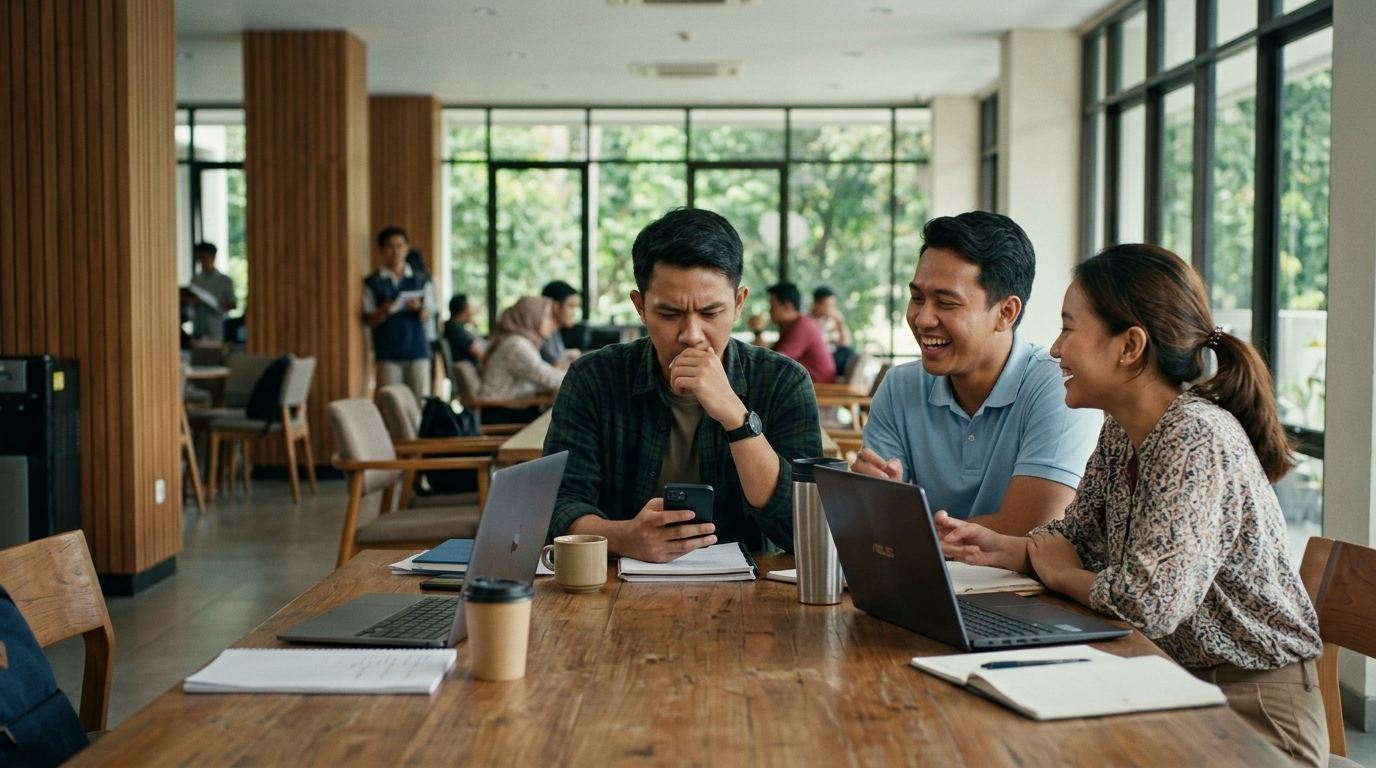
\includegraphics[width=\linewidth]{images/scene_2.jpg} & Rama duduk sendirian di sudut lounge, laptopnya terbuka menampilkan daftar lamaran kerja yang sepi respons. Rama menghela napas menatap layar HP-nya. & 9 dtk & Menyorot kesendirian dan beban pikiran lulusan baru \\
\hline
3 & Int & Over the Shoulder & Still & Ambience lounge & Layar smartphone Rama menampilkan chat WA mencurigakan & Kamera dari balik bahu menyorot pesan tawaran Admin WFH gaji 15 juta, namun wajib deposit seragam 500rb dan kirim selfie KTP. & 7 dtk & Focus pull dari bahu ke layar ponsel (crop jernih) \\
\hline
4 & Int & Close Up & Slow push-in & Monolog Rama & Wajah Rama membaca pesan dengan kening berkerut & \textbf{Rama (Monolog)}: ``Admin WFH gaji dua digit... Tapi kenapa baru tahap awal udah disuruh transfer lima ratus ribu buat uang seragam? Terus minta foto selfie KTP juga...'' & 12 dtk & Menyorot keraguan mendalam antara peluang dan kejanggalan \\
\hline
5 & Int & Medium Close Up & Still & Monolog Rama & Rama meletakkan HP di meja dan memegang keningnya & \textbf{Rama}: ``Aku udah empat bulan wisuda belum dapet kerja... Di satu sisi aku takut ini penipuan dan data KTP-ku disalahgunakan. Tapi di sisi lain, aku takut nolak kalau ternyata ini beneran rezeki. Pas kondisi lagi terdesak begini, susah banget buat mikir jernih...'' & 14 dtk & Menyorot fenomena nyata \textit{Job-Seeker Desperation Bias} \\
\hline
6 & Int & Close Up to Med & Still & Monolog Rama & Rama mengambil HP dan berkasnya, beranjak berdiri & \textbf{Rama}: ``Nggak, aku nggak boleh gegabah ambil keputusan pas lagi panik. Mumpung lagi di kampus, lebih baik aku konsultasikan hal ini ke Pak Ganjar di ruang dosen.'' & 8 dtk & Sikap proaktif mencari verifikasi objektif ke dosen \\
\hline
7 & - & Split Screen & Still & Voiceover Hafidz & Layar kiri: B-roll Rama melangkah keluar lounge. Layar kanan: Kartu infografis data bersih & \textbf{Hafidz (VO)}: ``Data BPS mencatat lebih dari 7,2 juta pencari kerja di Indonesia. Riset GASA membuktikan 49\% penipuan berawal dari loker fiktif dengan kerugian Rp49 triliun. Dalam tekanan ekonomi, bias keputusasaan melumpuhkan logika kritis korban.'' & 20 dtk & Infografis 2D minimalis elegan (tanpa 3D orbit) \\
\hline
8 & - & Full Screen & Fade in & SFX Sub-bass whoosh & Title card elegan: VERIFIN: Garda Talenta Digital & Teks bersih pada dark navy: \newline \textbf{VERIFIN: GARDA TALENTA DIGITAL} \newline \textit{Sistem Deteksi Loker Palsu Berbasis AI \& Multi-Source OSINT} \newline Three Achilles -- TRPL SV UGM & 9 dtk & Title reveal profesional dan berwibawa \\
\hline

\multicolumn{9}{|c|}{\cellcolor{gray!10}\textbf{BABAK II: THE BRIDGE \& COGNITIVE INTERVENTION (01:45 -- 02:45)}} \\
\hline
9 & Int & Medium & Track in & Ambience tenang & Rama mengetuk dan memasuki ruang dosen TILC & Rama berkonsultasi mengenai tawaran kerjanya kepada Pak Ganjar di ruang dosen. & 9 dtk & Framing rapi di ruang kerja dosen \\
\hline
10 & Int & Two Shot & Still & Dialog Rama \& Pak Ganjar & Pak Ganjar dan Rama duduk berhadapan & \textbf{Rama}: ``Saya bimbang banget, Pak Ganjar. Format pesannya rapi mencatut nama perusahaan besar, tapi mereka mewajibkan transfer uang registrasi. Saya takut salah ambil keputusan karena panik butuh kerja.'' & 10 dtk & Dialog konsultasi hangat dosen-mahasiswa \\
\hline
11 & Int & Medium Close Up & Still & Dialog Pak Ganjar & Pak Ganjar tersenyum menenangkan dan memberi arahan solusi\par\vspace{3pt}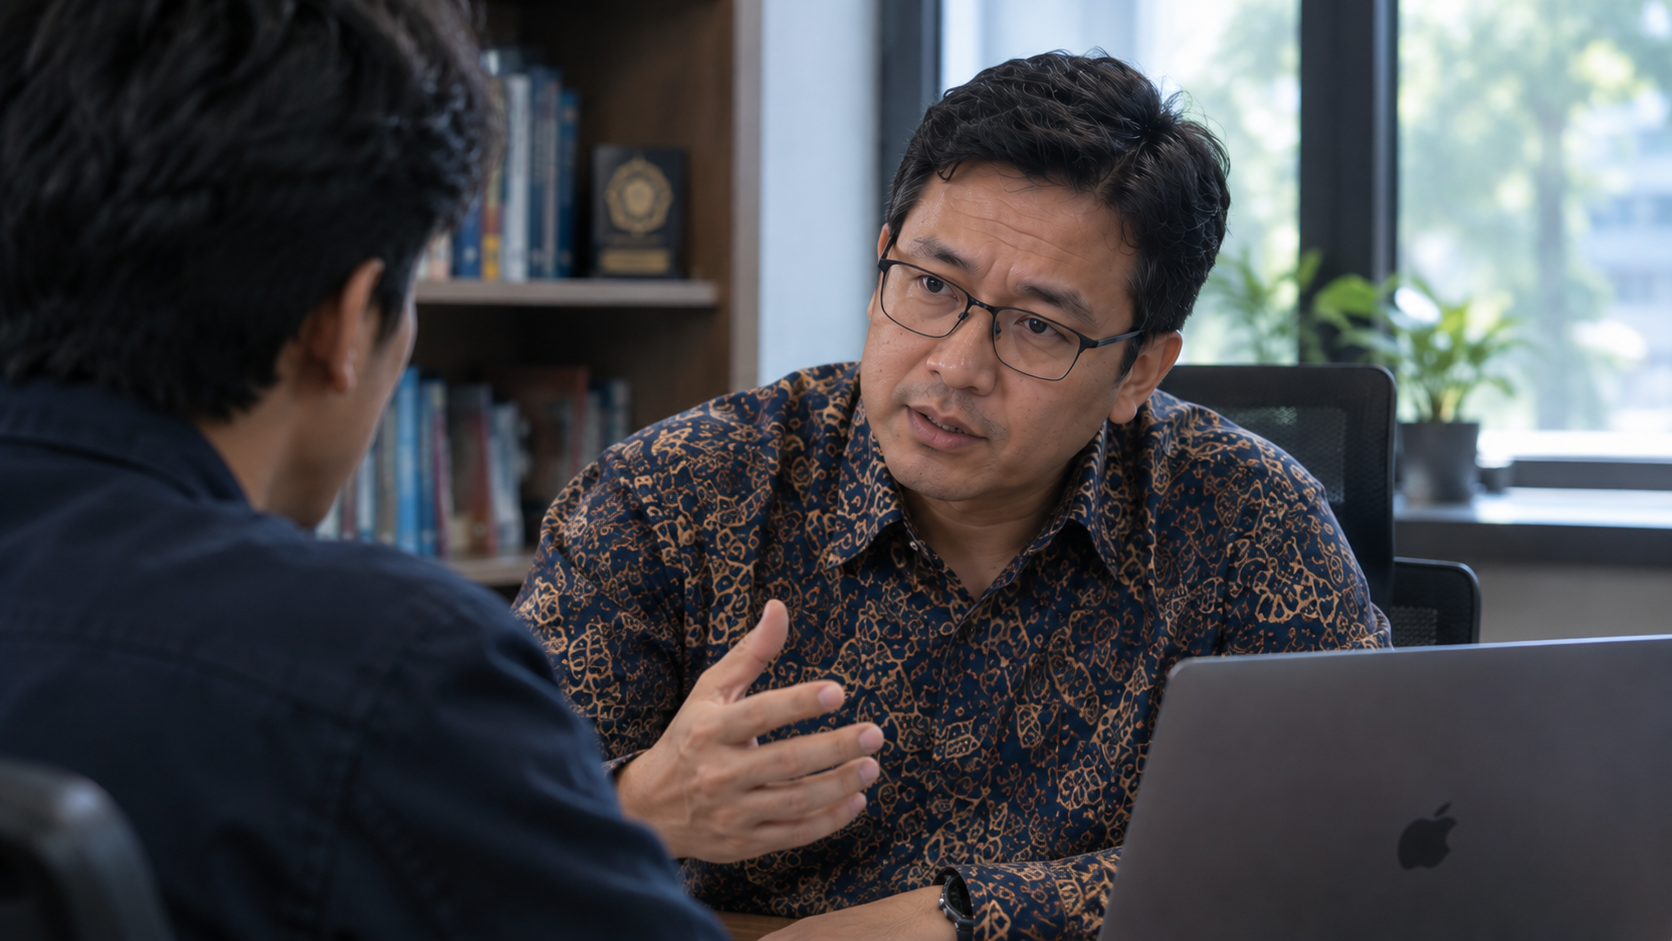
\includegraphics[width=\linewidth]{images/scene_12.png} & \textbf{Pak Ganjar}: ``Keputusan kamu tepat untuk berhenti sejenak dan tidak langsung transfer, Rama. Sindikat memang mengeksploitasi kepanikan pelamar. Kamu butuh bukti forensik digital objektif. Rekan-rekanmu di TRPL SV UGM sudah meluncurkan \textbf{Verifin} sebagai jeda kognitif berbasis AI dan OSINT. Sistemnya sudah live 100\%, ayo kita uji langsung di lab.'' & 25 dtk & Menghubungkan konsep psikologi ke teknologi \\
\hline
12 & Eks & Medium & Tracking walk & Ambience selasar & Pak Ganjar dan Rama berjalan di selasar lantai 2 TILC & Pak Ganjar dan Rama berjalan melintasi selasar modern kampus TILC menuju Lab Rekayasa Perangkat Lunak. & 8 dtk & Transisi dinamis menghubungkan dua lokasi \\
\hline
13 & Int & Wide & Pan left & Ambience lab & Lab Software Engineering TRPL SV UGM & Workstation dual-monitor aktif. Hafidz, Matthew, dan Akmal sedang berdiskusi kode dan menyambut Pak Ganjar serta Rama dengan ramah. & 14 dtk & Menampilkan ruang lab riil dan kesiapan tim \\
\hline

\multicolumn{9}{|c|}{\cellcolor{gray!10}\textbf{BABAK III: THE BATTLE OF EDGE CASES -- LIVE DEMO 100\% (02:45 -- 06:15)}} \\
\hline
14 & Int & Over the Shoulder & Still & Dialog Tim \& Rama & Rama duduk di depan workstation, Matthew mendampingi & \textbf{Matthew}: ``Kunci Verifin adalah memutus bias emosional dengan transparansi bukti forensik. Mas Rama dapat tawaran lewat mana? Kita langsung salin teks dan tautannya ke sistem!'' \newline \textbf{Rama}: ``Ini Mas, ada dua kasus ekstrem yang bikin aku bingung. Pertama broadcast BUMN besar ini.'' & 14 dtk & Menyiapkan uji komparasi dua kasus ekstrem \\
\hline
15 & Int & Screen Capture & Still & SFX Typing \& Klik & Layar browser live verifin.app (Next.js 16) & Rama menempelkan teks chat BUMN Semen Indonesia dan link recruitment-semenindonesia.xyz ke kolom form Verifin lalu menekan tombol ``Analisis Lowongan''. & 11 dtk & Screen recording jernih 1080p 60fps \\
\hline
16 & - & Screen Capture & Still & SFX Alert Ping & Dashboard Hasil: Trust Score Gauge berputar ke 94/100 (Badge Merah)\par\vspace{3pt}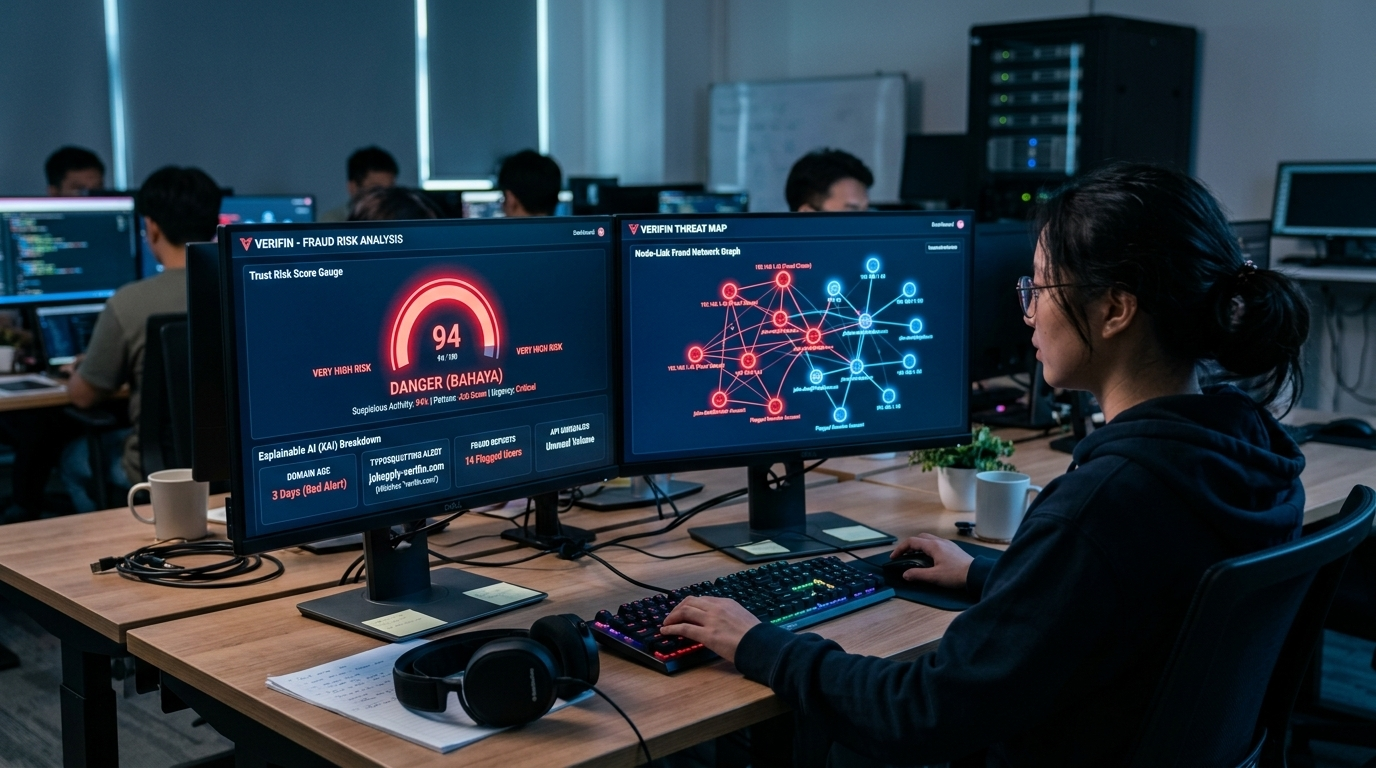
\includegraphics[width=\linewidth]{images/scene_20.jpg} & Tampil dashboard hasil instan dalam 1,8 detik. Skor Risiko 94/100 (BAHAYA TINGGI - WASPADA PENIPUAN). \newline Kartu Bukti XAI Merah: \newline $\bullet$ Domain Age: 5 Hari (Penalti +30) \newline $\bullet$ Typosquatting .xyz vs Resmi .co.id \newline $\bullet$ Biro Travel: 14 Laporan Fraud di Kredibel.id & 15 dtk & Worst-Case FAKE terbongkar tuntas secara ilmiah \\
\hline
17 & Int & Medium & Still & Dialog Matthew \& Rama & Matthew menunjuk rincian bukti forensik digital pada monitor\par\vspace{3pt}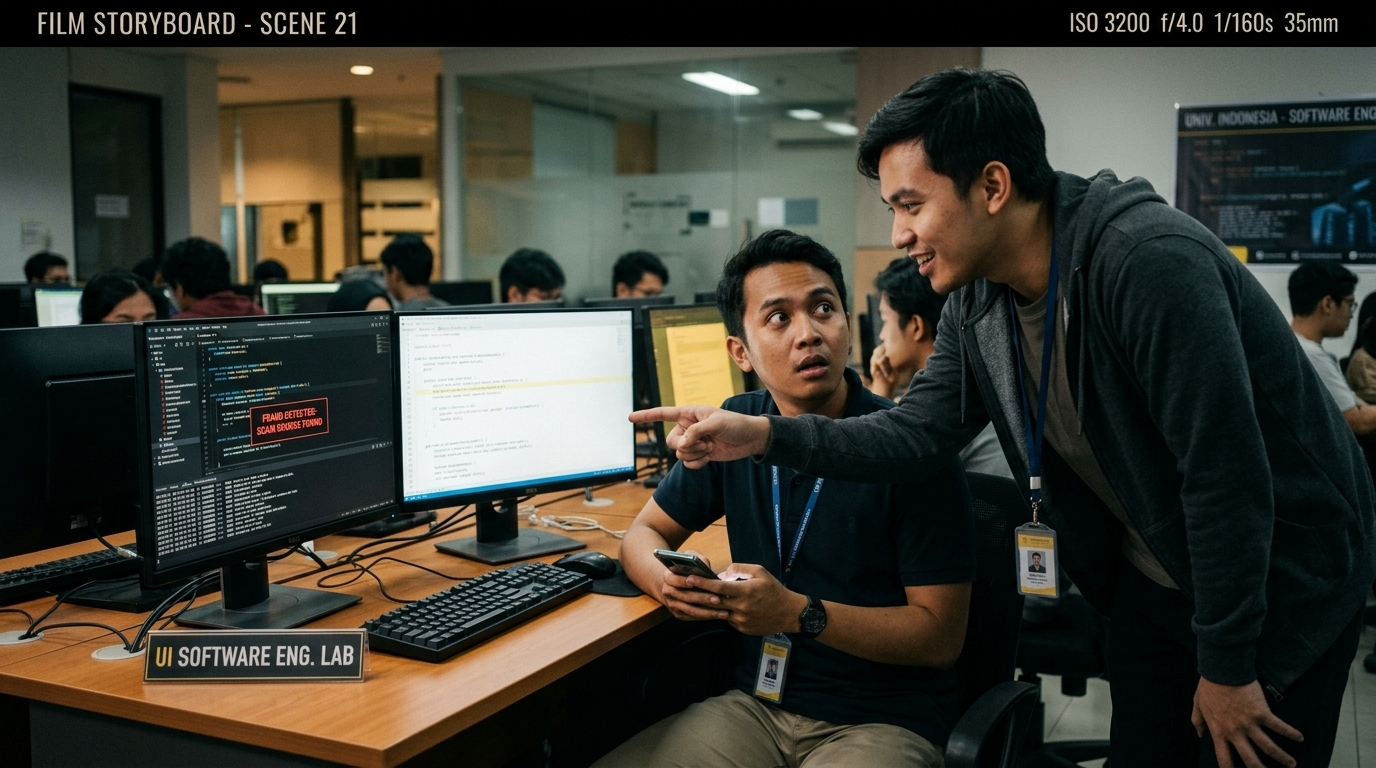
\includegraphics[width=\linewidth]{images/scene_21.jpg} & \textbf{Matthew}: ``Perhatikan bukti forensiknya Mas Rama. Format WA terlihat resmi, tapi mesin OSINT Verifin membongkar domain ini baru berumur 5 hari, memakai ekstensi .xyz murah, dan kontak biro travelnya sudah memiliki 14 laporan penipuan tiket di Kredibel!'' \newline \textbf{Rama}: ``Ya ampun... Kalau tadi aku cuma percaya format teks rapi doang, uangku pasti langsung ludes buat tiket fiktif!'' & 25 dtk & Dialog tajam membongkar modus penipuan \\
\hline
18 & Int & Screen Capture & Pan / Click & SFX Click Tab & Tab Fraud Network Graph dibuka & Kursor mengklik tab Fraud Network Graph. Graf interaktif (React Flow + D3.js) menampilkan node nomor telepon penipu menyala merah dan terhubung ke 3 sindikat PT fiktif lainnya di database. & 18 dtk & Bukti intelijen data grafis sindikat riil \\
\hline
19 & Int & Medium & Still & Dialog Hafidz & Hafidz menjelaskan kecerdasan graf sindikat & \textbf{Hafidz}: ``Verifin tidak bekerja terisolasi. Melalui Fraud Network Graph, sistem memetakan korelasi entitas. Nomor ini terbukti terkoneksi ke sindikat penipuan yang sama di beberapa kota dengan modus tiket serupa.'' & 16 dtk & Penjelasan kecerdasan graf lintas platform \\
\hline
20 & Int & Close Up & Still & Dialog Rama & Rama menunjukkan chat kedua di ponselnya & \textbf{Rama}: ``Bener-bener membuka mata aku... Tapi gimana dengan kasus kedua ini Mas? Ada broadcast loker toko motor lokal di Jogja (The Biker Shop), tapi daftarnya lewat Google Form dan emailnya cuma Gmail gratisan (hrdthebikershop@gmail.com). Ini penipuan juga?'' & 16 dtk & Memulai pengujian kasus kedua: Anti-False Positive \\
\hline
21 & Int & Screen Capture & Still & SFX Processing & Teks loker The Biker Shop di-paste ke Verifin & Teks broadcast loker The Biker Shop disalin dari HP dan diinput ke Verifin. Tombol analisis diklik. & 6 dtk & Pengujian cepat kasus UMKM lokal \\
\hline
22 & - & Screen Capture & Still & SFX Success Ping & Dashboard Hasil: Skor Risiko 12/100, Badge Hijau (AMAN \& TERVALIDASI) & Tampil kartu callout XAI warna hijau lembut: \newline $\bullet$ Alamat Fisik Valid: Jl. Parangtritis No. 38 (OpenStreetMap) \newline $\bullet$ Medsos Aktif: IG @thebikershop.jogja (1.6K Followers) \newline $\bullet$ Klausul Finansial: Bebas Biaya (Penalti 0) & 16 dtk & Anti-False Positive terbukti nyata di antarmuka \\
\hline
23 & Int & Medium & Still & Dialog Akmal \& Hafidz & Akmal dan Hafidz menjelaskan di depan monitor & \textbf{Akmal}: ``Inilah inovasi Anti-False Positive Verifin. Sistem kami tidak sembarangan memvonis merah hanya karena email Gmail. Mesin OSINT memverifikasi toko fisiknya nyata di Jalan Parangtritis via OpenStreetMap dan medsosnya aktif berniaga.'' \newline \textbf{Hafidz}: ``Dengan begitu, UMKM lokal terlindungi dan pencari kerja tidak kehilangan kesempatan kerja yang sah.'' \newline \textbf{Rama}: ``Wah, adil banget! Jadi aku nggak perlu ragu lagi buat melamar!'' & 25 dtk & Nilai inovasi keadilan sistem (Fairness \& Trust) \\
\hline
24 & Int & Screen Capture & Still & SFX Shutter & Pengujian Kanal Input Gambar OCR & Matthew mendemokan kanal gambar: Screenshot poster loker buram diunggah. Engine PaddleOCR 2.8 mengekstrak teks otomatis dan menganalisis risiko dalam hitungan detik. & 18 dtk & Demo fleksibilitas input multimodal (Screenshot HP) \\
\hline
25 & Int & Screen Capture & Still & SFX Click FAB & Tombol Floating Action Button ``[!] Laporkan Loker'' diklik & Kursor mengklik FAB oranye kontras di pojok kanan bawah. Form pelaporan terisi otomatis dan tersinkronisasi ke Community Feed Real-Time untuk melindungi sesama pelamar. & 17 dtk & Demo pertahanan komunitas hasil evaluasi testing \\
\hline

\multicolumn{9}{|c|}{\cellcolor{gray!10}\textbf{BABAK IV: SOFTWARE ENGINEERING EXCELLENCE \& VALIDASI (06:15 -- 07:55)}} \\
\hline
26 & Int & Medium Two Shot & Still & Dialog Hafidz \& Matthew & Hafidz dan Matthew memaparkan arsitektur di depan monitor lab & \textbf{Hafidz}: ``Di balik kemudahan antarmuka, Verifin mengusung arsitektur multi-layer tangguh: Layer 1 Hybrid NER, Layer 2 Fast NLP Classifier, Layer 3 Parallel Async OSINT, Layer 4 Graph Reasoning, dan Layer 5 Additive Explainable AI. Setiap skor dihitung transparan dari temuan bukti forensik digital, bukan sekadar asumsi model kotak hitam.'' & 28 dtk & Penjelasan arsitektur murni di lab tanpa 3D CGI \\
\hline
27 & - & Screen Capture & Still & SFX Typing Terminal & Rekaman layar eksekusi automated test \& metrik rekayasa & $\bullet$ Automated test: pytest tests/ $\rightarrow$ \textbf{100\% PASSED} (Coverage 91\%) \newline $\bullet$ Model ML: ROC-AUC mencapai \textbf{0,996} pada dataset EMSCAD \newline $\bullet$ Latensi respons FastAPI di bawah 2 detik \newline $\bullet$ Live deployment terisolasi di Dokploy \& Cloudflare Tunnel & 22 dtk & Pembuktian software engineering tangguh \& riil \\
\hline
28 & Int & Medium & Still & Dialog Akmal \& Matthew & Akmal dan Matthew memegang dokumen pengujian \& kemitraan prodi & \textbf{Akmal}: ``Aplikasi telah melalui usability testing terstruktur pada pencari kerja muda untuk memastikan antarmuka bebas friksi.'' \newline \textbf{Matthew}: ``Kredibilitas sistem kami tervalidasi melalui kerja sama resmi dengan Prodi TRPL SV UGM, di mana Verifin diimplementasikan sebagai modul kurasi loker bagi calon lulusan dan alumni.'' & 22 dtk & Validasi empiris pengguna \& kemitraan institusi kampus \\
\hline

\multicolumn{9}{|c|}{\cellcolor{gray!10}\textbf{BABAK V: RESOLUTION, EMPOWERMENT, \& CLOSING CALL (07:55 -- 08:50)}} \\
\hline
29 & Int & Two Shot & Still & Dialog Pak Ganjar & Pak Ganjar menepuk bahu Rama di Lab RPL dan tersenyum bangga\par\vspace{3pt}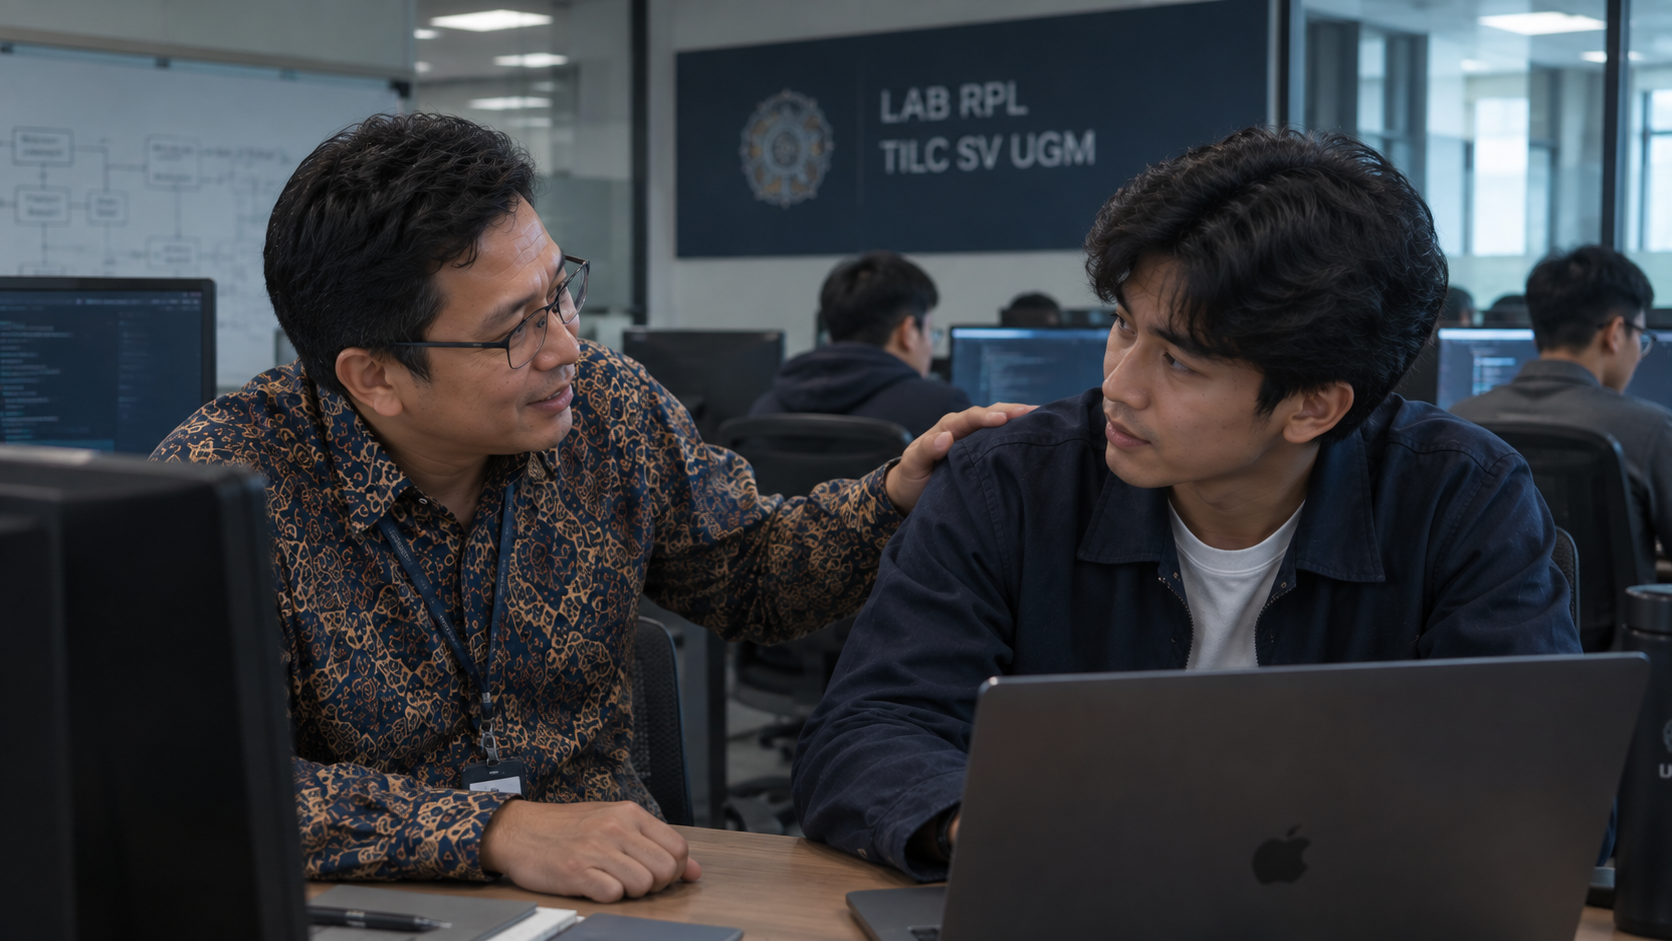
\includegraphics[width=\linewidth]{images/scene_35.png} & \textbf{Pak Ganjar}: ``Kerja keras yang luar biasa Three Achilles. Verifin membuktikan bahwa rekayasa perangkat lunak hadir sebagai instrumen penyelamat nyata, mengembalikan akal sehat dan melindungi masa depan talenta muda Indonesia.'' & 15 dtk & Apresiasi akademis \& etika profesi rekayasa \\
\hline
30 & Int & Close Up & Still & Dialog Rama & Rama membuka web Verifin di browser smartphone-nya & \textbf{Rama}: ``Terima kasih banyak Pak Ganjar dan tim Verifin! Sekarang rasanya bener-bener plong dan aman. Cukup sekali cek di Verifin, aku bisa melamar kerja dengan tenang tanpa takut terjebak penipuan.'' & 13 dtk & Resolusi kepraktisan mobile web \& ketenangan batin \\
\hline
31 & Eks & Medium Tracking & Slow dolly back & Music Up (Heroic) & Kelima pemeran melangkah di selasar megah TILC SV UGM\par\vspace{3pt}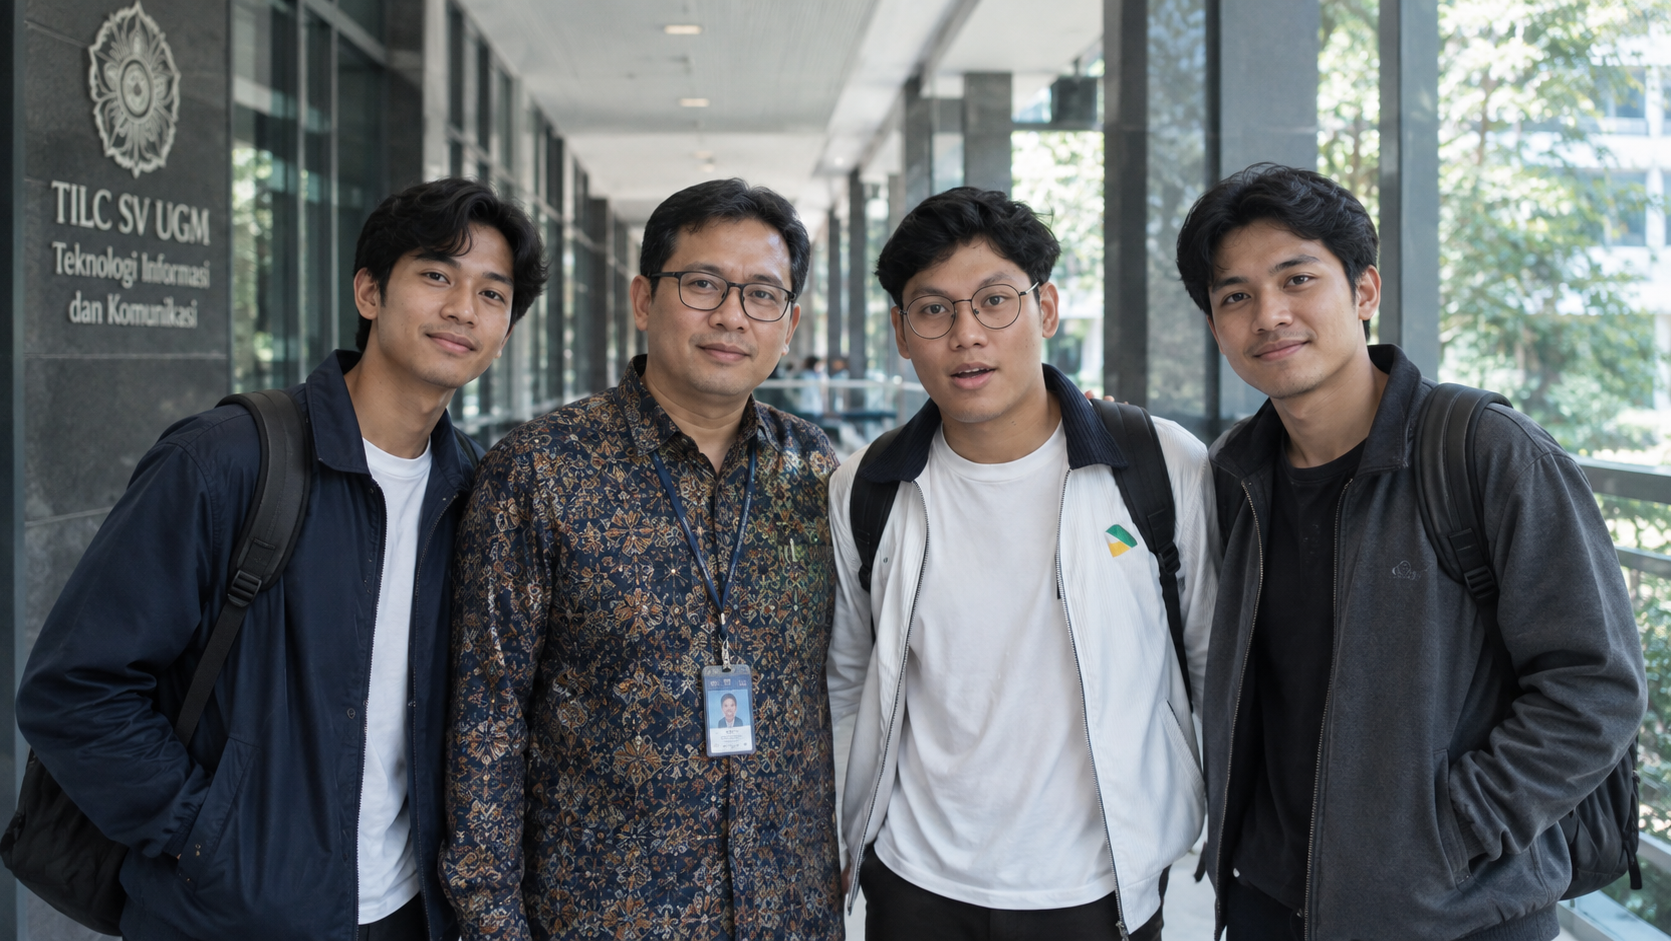
\includegraphics[width=\linewidth]{images/scene_37.png} & Kelima pemeran (Rama, Pak Ganjar, Hafidz, Matthew, Akmal) mengenakan jas almamater UGM melangkah mantap di selasar kampus megah di bawah sinar matahari hangat. & 10 dtk & Visual sinematik klimaks kampus \\
\hline
32 & Eks & Medium & Still & Orasi Penutup Tim & Kamera menyorot kelima pemeran & \textbf{Hafidz}: ``Bagi jutaan pemuda Indonesia, lowongan kerja adalah gerbang masa depan, bukan perangkap keputusasaan.'' \newline \textbf{Matthew}: ``Verifin hadir sebagai garda terdepan, membentengi talenta bangsa dengan kecerdasan data dan transparansi.'' \newline \textbf{Akmal}: ``Sebuah karya rekayasa perangkat lunak dari Sekolah Vokasi UGM untuk Indonesia yang aman dan berdaya.'' \newline \textbf{Semua Bersama}: ``Kami Tim Three Achilles, siap mengawal talenta bangsa di GEMASTIK XIX 2026!'' & 27 dtk & Orasi penutup menggelegar dan solid \\
\hline

\multicolumn{9}{|c|}{\cellcolor{gray!15}\textbf{BUMPER PENUTUP}} \\
\hline
Outro & - & Full Screen & Still & SFX Chime \& Fade & Background Dark Slate Elegan & $\bullet$ Logo GEMASTIK XIX 2026 \& Universitas Gadjah Mada \newline $\bullet$ URL \& QR Code Live App: verifin.app \newline $\bullet$ Badge Emas: 100\% LIVE DEPLOYMENT \& OPEN REPOSITORY \newline $\bullet$ Credit: Tim Three Achilles -- D4 TRPL SV UGM 2026 & 10 dtk & Outro resmi penutup video karya final \\
\hline

\end{longtable}

\end{document}
